\mysection{The Abandoned}{forgotten-abandoned}

If the true name of one of the Forgotten is known, it can be used to call them forth from the edge of annihilation. These "remembered" Small Gods are known as the Abandoned - archons, seraphs, and fiends lost and buried in time. 

One of the names of the Abandoned exists in your memory when you first create your Spriggan Adventurer. If you know which Abandoned you want to serve you when you first begin, you can name them immediately - otherwise, you can name them at any point during the game, and they will appear in your time of need. Once you name your Abandoned, you cannot change - it is as if you had always known its name, and suddenly remembered it.  You can learn the names of additional Abandoned during \mylink{Advancement}{advancement}, or while adventuring - their names placed by the Arbiter on ancient jungle stela buried beneath rotting vines, inscribed on black amulets at the bottom of the sea, written on the bases of broken idols in forgotten tombs, etc.

You can summon one of the Abandoned simply by saying their name, but you can only summon each of them once per Session, and you can only summon one at a time. The Abandoned do not require your Concentration to exist. When one of the Forgotten Adjourns, they immediately wink out of existence. \mybold{Unless otherwise noted, the Abandoned will not Adjourn until the end of the Session!}  They can Adjourn of their own free will (but will rarely do so), and will obviously Adjourn if they are "killed". 

\cbreak

Keep in mind that unlike the Obliterated, the Abandoned have memory and personalities (the Arbiter is encouraged to treat them like a henchman or hireling), and won't take kindly to being forced to Adjourn by "killing" them!

Any attacks against the Abandoned automatically succeed. They can take your \MAX Sovereignty x 5 Health of damage (so if you have \MAX 3 Sovereignty, they have 15 Health). \mybold{If an Abandoned Adjourns for any reason during a Session, it will not return until the next Session}.

\begin{center}
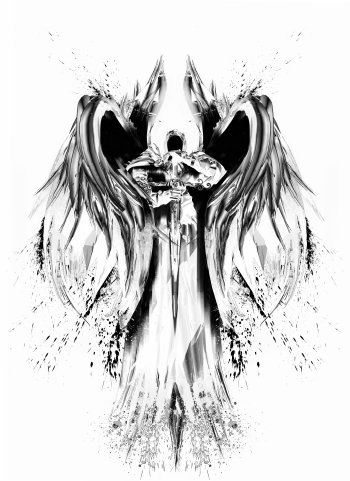
\includegraphics[scale=.5]{remembrance/Archon}
\end{center}

The Abandoned will try to remain Close to you (for you are the only reason they exist). They can move as fast as you move, no matter what the conveyance. If you are teleported for some reason, the Abandoned will continue to remain Close to you.  If you are knocked unconscious or incapacitated for some reason, the Abandoned will stay with you. If you are ever brought to 0 Flesh, the Abandoned will Adjourn in terror (for it's completely possible that the last creature to remember their name is about to die).


Below are the true names of 12 Archons, Seraphs, and Fiends. This is by no means a complete list!



\newpage
\end{multicols*}

\ed{"Remixed" from Skerple's mind-blowing \href{https://coinsandscrolls.blogspot.com/2019/10/osr-glog-based-homebrew-v2-many-rats-on.html}{GLOG Homebrew v.2}}

\mysubsection{The Archons}{forgotten-archons}

\myhighlight{Big Mac, "Good Time Guy"}{abandoned-big-mac-good-time-guy}

Big Mac crashes through a window or door and drunkenly hugs the first person he sees. He appears as a portly robed monk with a tankard of beer and a rosy complexion.  He is totally smashed and very happy.  

Unless Big Mac is at a party (at minimum, drinks and 2 happy people) he will leave the way he came in with an "Irish goodbye" (Adjourn).  If there's a party, he will continue to drink from his tankard (which never gets empty), tell tall tales, reminisce, propose mad schemes, sing songs in all languages, provide terrible advice, and sometimes throw up.  He cheers up any low-class social event and scandalizes anyone tasteful. Big Mac can find a number of items equal to your Sovereignty for you, provided they are party related.  Examples:  more beer, a safe place to crash, a person of negotiable virtue, Pooka, narcotics, musicians.  He can remove Toxins or Drunkeness from a number of people equal to your Sovereignty.

\myhighlight{Bon Chapeau, Hat of Marvels}{abandoned-bon-chapeau-hat-of-marvels}

Bon Chapeau enters with a burst of light on a Close or Nearby target's head you specify (including your own).  It appears as a magnificent hat, crown, turban, etc. depending on how Bon Chapeau is feeling that day (but it will always match the wearer's garments). Once Bon Chapeau attaches to someone's head, he'll refuse to move for any reason; however, if the wearer of Bon Chapeau moves more than Far Away from you, Bon Chapeau will Adjourn.

If the wearer is under any negative effects of the mind when Bon Chapeau appears on their head, the effects immediately end. This can include the \mylink{Secrets of the Mind}{arcana-wizardry-secrets-alignment} and \mylink{Madness!}{injury-insanity-madness}. If someone attempts to perform a Secret of the Mind against the wearer, the spell immediately rebounds upon the caster. 

The hat can hear the wearer's thoughts, and will tell them to you if you ask nicely.   Finally, Bon Chapeau can also judge fashion shows; tell you if your outfit is flattering; and know if an article of clothing is a knock-off or not just by smell.

\myhighlight{Bufo, the Lickable Toad}{abandoned-bufo-the-lickable-toad}


A fat, polychromatic, four-eyed toad the size of a cow hops in from around the corner. He has eyes like a starry sky, numerous oozing postules, and speaks in a booming croak.

Anyone who licks Bufo must make an \mylink{Insanity}{adventurer-kismet-insanity} try; if they succeed, they can invoke one of the following effects:

\callout{\footnotesize{
\mybullet {
    \item They can restore all the facets of their \mylink{Personality}{adventurer-personality} to their \MAX;
    \item They can heal their Flesh fully; or   
    \item They can heal their Grit fully.
}}}

\begin{wrapfigure}[11]{l}{0.4\textwidth}
    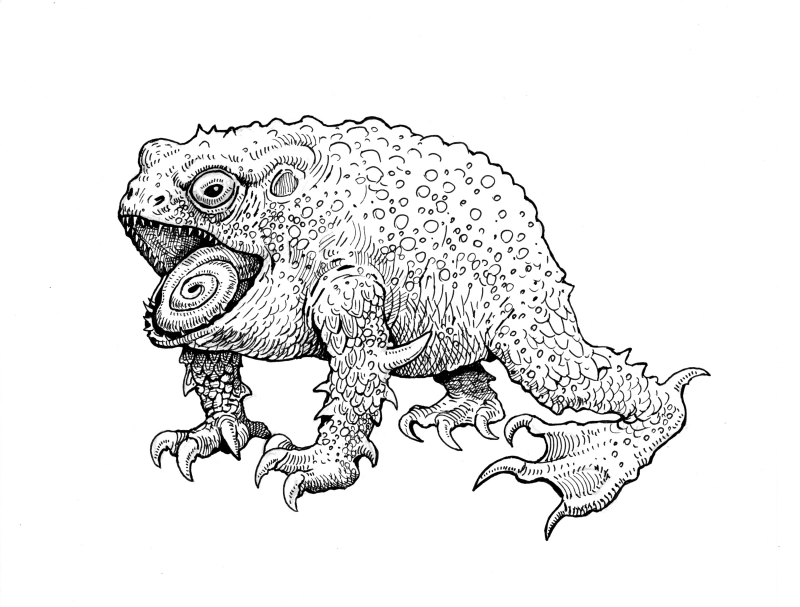
\includegraphics[width=0.4\textwidth]{remembrance/BufoTheToad}
\end{wrapfigure}



Bufo doesn't like being licked; you or your Allies can only lick him a number of times equal to your Sovereignty; after that, no further beneficial effects can occur for the remainder of the Session.



Bufo can swallow up to 25 Burden worth of objects or gear. Objects swallowed by Bufo enter \mylink{Hammerspace}{meta-hammerspace} until he Adjourns; just before he disappears, he will spit them back out.  He'll only swallow things that look delicious (but he's easily tricked).  The object swallowed can't be bigger than he is.


\myhighlight{Gemma, Translator of Mysteries}{abandoned-gemma-translator-of-mysteries}

A thin, tired woman with wiry hair appears wherever you're not looking. Gemma can speak and translate any language (living or dead), and will translate for you in real time. She can also read (and translate) texts written in any language, but she won't translate "blasphemies" (Arbiter's discretion). If you hand Gemma a \mylink{Fetish}{fetishes} or \mylink{Grimoire}{grimoires}, she can cast spells from them using a number of d4 equal to your Sovereignty. These dice act in all ways like \mylink{Blood Dice}{cruces-blood} (roll any number of dice in your pool; dice disappear on Failure; rolling triples, quadruples, and quintuples is "bad", etc.). If Gemma runs out of dice, she Adjourns. Secrets read from Fetishes or Grimoires are immediately destroyed (in the case of a Fetish) or erased (in the case of a Grimoire). Gemma can read a \mylink{Sigil}{research-inscription-sigils} without activating its effects (and tell you what it is).

Gemma can't (or refuses to) write.  While she is Close to you, you can't be \mylink{Befuddled}{effect-befuddled} (and ends any Befuddled effect on you if applicable). She will Adjourn if a book is burned in her presence, but will remember it the next time she comes ...

\myhighlight{Istv{\AccentA}n, the Lost}{abandoned-istvan-the-lost}

A tired, middle-aged man with blue eyes shuffles in politely. Name a destination to Istv{\AccentA}n. Anyone who talks to Istv{\AccentA}n will give him directions to that destination.  Directions given will be to the best of the person's knowledge, and can include the location of treasure, traps, hazards, patrols, etc. etc.  Ask a peasant how to get to the moon and he'll shrug and suggest a mountain; ask the Grand Archmage of the Isle of Carcosa and you might get a very different answer. Any direction given to Istv{\AccentA}n will either get you to your goal, or get you closer to your goal.

If you follow Istv{\AccentA}n anywhere, he will always get you to your destination by the most circuitous (and potentially dangerous) route the Arbiter can imagine. If you reach the end of the Session and haven't arrived at your destination, Istv{\AccentA}n gives you directions before he Adjourns. These directions will get you where you need to be but (again) by the most circuitous (and potentially dangerous) route the Arbiter can imagine.


\myhighlight{Judyth, the Tiebreaker}{abandoned-judyth-the-tiebreaker}

Judyth is a floating stone sphere about bowling ball sized, carved in the shape of a human head.  She floats down from the ceiling and speaks with a decisive, stern voice.  If two objects, items, ideas, or issues are presented to Judyth (along with some criteria for judging) she will judge their merits. For example, you could ask "Which of these gems is most valuable?", "Which of my friends loves me most?" or "Which of these two mushrooms is poisonous?" Judyth can't answer questions that aren't local and immediate:  "Which country will win the war?" or "Which hallway did the thief run down?" aren't allowed, for example.  

If Judyth is presented with a paradox, she will immediately Adjourn in a logic bomb that deals your Sovereignty x2 damage to everyone Close (Save for half), except you.

\myhighlight{Mikhael, the Justifier}{abandoned-mikhael-the-justifier}

A middle-aged, completely bland man enters with a shuffle.  You can't really describe him further than that; his appearance seems to be easily forgotten, as if he were completely grey or beige. Mikhael will sidle up just behind anyone you specify (up to a distance of Nearby) and whisper in their ear in a low and soothing voice, helping them justify any scheme and freeing them of any guilt or doubt concerning it. Alternately, he can convince them of any plan you specify to him, provided the plan doesn't physically harm anyone (Arbiter's discretion).

While Mikhael is Close to you, you are both immune to \mylink{Murder}{vulgate-whispers-murder} and \mylink{the Drop}{combat-drop}. Any arrows or projectiles aimed at you or Mikhael automatically miss. 


\myhighlight{Mon Signor, the Deliverer}{abandoned-mon-signor-the-deliverer}

A bellboy wearing a red fez comes sprinting in with a patter of feet. He gives a quick bow and then waits expectantly for you to hand him something. The object you give him can be up to the size of a human body. The moment you hand him something, he immediately Adjourns.

The next time you summon Mon Signor, he will give you back the item you gave him previously, and wait expectantly for a tip (optional).  The returned item exists as if no time passed (it endures outside of Hammerspace; for all intents and purposes, the item/body/whatever is removed from the game until Mon Signor returns). If you hand an item to Mon Signor again (the same or a different object), he will immediately Adjourn with the item and return it next time he is summoned.

Unwilling "items" being handed to Mon Signor get a Save.

\myhighlight{Randy. Just Randy}{abandoned-randy-just-randy}

A pop, a short scream, and Randy falls down from the ceiling.  He is an acned teenage human with an imperious air, brown hair stuffed beneath a tattered pointed hat decorated with stars and moons, and a torn blue robe tied with a belt.  Randy was once a wizard's apprentice; a botched spell trapped him in a pocket dimension where he lives on, immortal and extremely confused. He is perpetually being dragged into combat, danger, dismemberment, and extremely awkward situations. He refuses to move further than Far-Away from you (and if you somehow force him outside of this range, he'll reappear Close to you, falling down from the ceiling).

Randy will sort-of obey you for the Session, but he is only an immortal teenager. He's awful at everything. If you want, you can direct any physical attack against you to Randy instead (provided Randy is Close to you).  If you have more than 3 Sovereignty, Randy's efforts are accompanied by appropriately dismal music.  Randy insists on an honorific i.e. "Randy the Magnificent", "Randy the Stupendous", etc. but no one ever calls him that.

\myhighlight{Sm{\UmlautO}k, the Grey Messenger}{abandoned-smok-the-grey-messenger}

Sm{\UmlautO}k seeps in through cracks in the floor and ceiling, appearing as a grey flag flapping in the wind. You can give Sm{\UmlautO}k a message containing a number of words equal to your Sovereignty, or an item smaller than an apple. You can designate any point you have ever seen, or any member of your Band (past or present), and Sm{\UmlautO}k will move "with the speed of an arrow" (Aribiter's discretion) to bring the message or item to the location or person you designated. If given an item, it becomes part of Sm{\UmlautO}k while it travels. Treat Sm{\UmlautO}kas sentient ... ah, smoke ... if you need to figure out whether or not Sm{\UmlautO}k can reach its target. A strong wind won't kill Sm{\UmlautO}k, but it will certainly slow it down.

As soon as the item is delivered, Sm{\UmlautO}k Adjourns. If Sm{\UmlautO}k can't reach the target by the end of the Session, it will drop the item somewhere along the quickest path.


\myhighlight{VVulf, Trapfinder}{abandoned-vvulf-trapfinder}

The sound of a trap springing shut echoes through the room, and a starving 3-legged wolf appears before you, fur matted with blood. VVulf will remain Close to you, padding alongside like a faithful hound. You cannot command him to move further than Close to you. When he is Close to you, you always win \mylink{Init}{combat-init}, you can are immune to \mylink{the Drop}{combat-drop} and you can automatically detect any traps Close or Nearby to you. This includes plots (for example, someone leading you into an ambush) but not lies.

Monsters with the Zoological Trait feel an affinity with VVulf. Provided combat has not been initiated, the Monster will not attack if they fail a Morale check.  VVulf is able to talk to mundane animals and ask simple questions (and receive basic answers).  

If you were to receive a blow that would bring you to 0 Flesh, VVulf will take the damage instead, and immediately Adjourn.  He can be forced to Adjourn by exhibiting cruelty to an animal, but he will remember ...

\myhighlight{Weeble, the Wobbling Stone}{abandoned-weeble-the-wobbling-stone}

A stone egg of a rotund, happy man with a cheerful grin appears in your hand. You can hand Weeble to another Ally if you choose, but Weeble cannot move further than Far-Away from you. The person holding Weeble cannot be knocked off their feet for any reason (including being knocked Prone, Stunned, the Vapors, etc) save death. Weeble also prevents you from falling - if you would fall into a pit or off a cliff, Weeble wobbles you back to safety at the last possible moment - but Weeble can't help you if the bridge collapses or your boat explodes or what-have-you.  If you dip Weeble into any liquid (soup, wine, etc) he will neutralize any \mylink{Toxins}{malignants-toxins} inside.

Weeble will Adjourn if he is tipped over and held down for a full minute. He hates this ... a lot. 


\mysubsection{The Fiends}{forgotten-fiends}


\myhighlight{Al'Ana, the Slaughtercaller}{abandoned-al-ana-the-slaughtercaller}

A red stone carved with a snarling tiger biting its own tail appears with a sizzle in your hand.  All iron weapons Close or Nearby Al'Ana deal double damage (both to Allies and Monsters).  You can whisper to Al'Ana and she will pounce at any Nearby or Far-Away target, striking unerringly and dealing your Sovereignty in damage (she will simply drop to the ground after striking her target). Al'Ana growls before ambushes, making you immune to \mylink{the Drop}{combat-drop}.

Al'Ana will willingly Adjourn if she is soaked in the viscera of a Monster or Ally who died in the confrontation she was just a part of.

\myhighlight{Ben Sidhe, Singer of Death}{abandoned-ben-sidhe-singer-of-death}

\begin{wrapfigure}{r}{0.5\textwidth}
    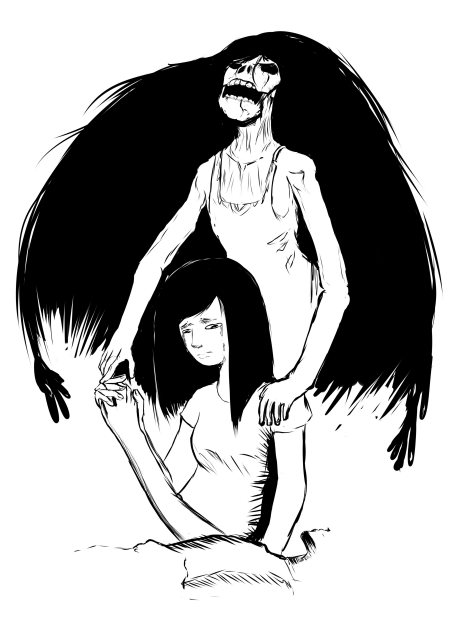
\includegraphics[width=0.48\textwidth]{remembrance/Banshee}
\end{wrapfigure}


A spectral woman with long, streaming hair boils up from the floor in a white mist.  She wears a grey cloak over a green dress; her hair is cast over her face, but you can see her eyes are red from weeping.  She immediately begins wailing.  All Nearby Monsters and Allies (except you) must \SAVE{Doom}or take your Sovereignty in damage.  The damage increases by +1 and repeats at the top of each Moment after the first (so if your Sovereignty were 3, Ben Sidhe would deal 3 damage, then 4 damage at the top of the next Moment, 5 damage at the top of the Moment after that, etc.).  The victims are always allowed a \SAVE{Doom} to take no damage, but they must try the Save \myital{each time}. Just as the damage increases by +1 each Moment, the \SAVE{Doom} try gets a +1 modifier each Moment (so victims would get a +1 on their Save in the second Moment, a +2 in the third, etc.)

Ben Sidhe cannot be silenced and will not stop weeping until she Adjourns.  She will always remain Close to you. She will weep for a number of Moments equal to your Sovereignty, and then Adjourn with a mournful echo.


\myhighlight{Diviser{\AccentE}, the Universal Chisel}{abandoned-divisere-the-universal-chisel}

A simple iron chisel with a wooden handle appears with a clang at your feet. Diviser{\AccentE} can move up to Far-Away instantly, but only when no one is looking at it. You can pick up and wield Diviser{\AccentE}, but if anyone else touches it Diviser{\AccentE} will reappear at your feet.

Diviser{\AccentE} excels at separating things. It can separate any two layers by touch (skin from muscle, gold foil from wood, rust from iron, the bark from a tree, etc.) provided they are fused together. It could not separate the armor from a warrior, for instance. It can separate things joined by \mylink{Brahe's Efficacious Sealant}{chymistry-brahes-efficacious-sealant}. This separation is not painless, where appropriate.

Further, Diviser{\AccentE} can drive a wedge between any two people that will last for the Session (if not beyond). The people must be no further than Nearby, and the two parties must be touched by Diviser{\AccentE}. This "wedge" will cause division, hard-feelings, suspicion, etc. at the mundane level, and also break Charm spells (though it cannot sever the bond between Vassal and Suzerain forged by the \mylink{Miracle:Covenant}{miracle-covenant} or \mylink{Miracle:Crusade}{miracle-crusade}). 

Diviser{\AccentE} can separate a number of things equal to your Sovereignty before it Adjourns. Each pair counts as one "thing", so separating skin from muscle only counts as 1 (but if you were to further separate muscle from bone, that would count as another "thing").


\myhighlight{Doppel, the Mirror}{abandoned-doppel-the-mirror}

Doppel can only be summoned by gazing into a full-length mirror or reflective surface (a still pool of water is OK, as long as it reflects your entire self). An identical duplicate steps from the surface, though with one minor difference (a different eye color, ram's horns instead of antlers, etc.) Doppel can move up to Far-Away from you. You have a complete telepathic connection with Doppel; by Concentrating for a Moment, you can see what Doppel sees, hear what Doppel hears, and mentally communicate complex tasks to Doppel (though Doppel can't improvise). Doppel will attempt to fulfill the letter (rather than the spirit) of your commands to the best of its abilities, but because of its Fiendish nature it will often do so in a way you may not have intended. You can command Doppel to Adjourn at any time. 

If you are Concentrating when Doppel takes any damage, that damage is also applied to you.  Doppel is unable to speak.

\myhighlight{Gitgud, the Taunter}{abandoned-gitgud-the-taunter}


A skinny monkey in torn robes appears with a low whistle.  Gitgud has a toothy, sneering grin and tiny red eyes.  Gitgud will taunt any target you tell it to with capers, jeers, wails, and jokes.  He is really distracting and annoying.  The target must \SAVE{Doom} or immediately become \mylink{Enraged}{effect-enraged} and attack Gitgud, who will run away to taunt from a safe distance (up to Far-Away from you). Add +4 to your \mylink{Guard}{combat-guarding} tries when rolling for Gitgud. He can climb and perform simple tasks with a monkey's patience and skill.

\begin{wrapfigure}[26]{l}{0.5\textwidth}
    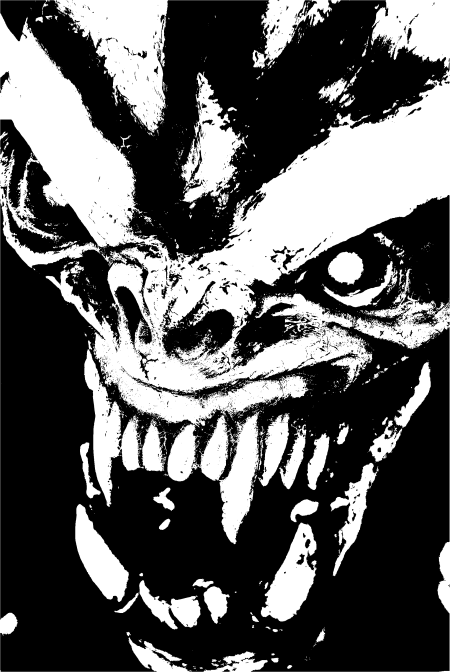
\includegraphics[width=0.48\textwidth]{remembrance/Demon}
\end{wrapfigure}


If Gitgud is not commanded to taunt a specific creature, or if that creature is slain, Gitgud will being taunting a random Ally or Monster (he'll taunt other Monsters first, then Mortals, then Unseelie). If you are the only creature around to taunt, he will Adjourn.

\myhighlight{Grendel, the Helping Hand}{abandoned-grendel-the-helping-hand}

A blue-green arm and hand drops from the sky with a wet thud.  The arm can be stuck to flesh and acts as an extra limb.  On a willing target, Grendel grants an additional \mylink{Unarmed}{combat-damage-unarmed} attack each Moment that deals \OneHalf your Sovereignty (rounded up) in damage.  Use the target's \FOC instead of \VIG or \DEX when they make their Attack try.  It can carry a shield or a lantern, or assist with climbing or swimming (+2 to the roll), but cannot wield a weapon.  If attached to an unwilling creature, Grendel will punch them in the nearest vulnerable spot, dealing \OneHalf your Sovereignty in damage. The arm detaches with a pop; it can be stuck to a number of creatures equal to your Sovereignty every Session before it Adjourns.

\newpage

\myhighlight{Grimalkin, Ruler of the Weak}{abandoned-grimalkin-ruler-of-the-weak}

A purring grey cat with yellow eyes comes slinking out from the shadows between your legs.  Grimalkin is an asshole; she'll ignore what your asking her, get into trouble, and generally be a nuisance.  However, she can also do the following at your command:

\callout{\footnotesize{
\mybullet {
    \item Eat a Curse (see \mylink{Hekaphage}{occultism-hekaphage});
    \item Turn any die roll that hits the table into a natural 1;
    \item Knock a single die off the (real world) table. The roller gets a re-roll;
    \item Find any Nearby secret door, trap, hidden object, or invisible object.
}}}

She can perform any of those abilities a number of times equal to your Sovereignty, at which point she Adjourns.

\myhighlight{Lucertola, the Taster}{abandoned-lucertola-the-taster}

\begin{wrapfigure}[15]{r}{0.5\textwidth}
    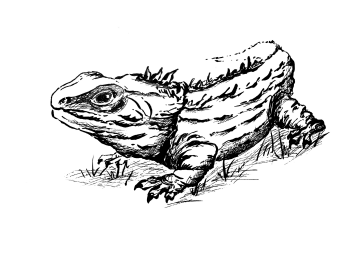
\includegraphics[width=0.48\textwidth]{remembrance/Lizard}
\end{wrapfigure}

A sleek yellow lizard with a bright blue tongue appears around your neck.  Lucertola can taste the air and tell you about the source of odors, smoke, fog, etc.  If you give Lucertola a taste of food or drink, she will tell you whether or not its safe to eat or drink.  While you're wearing Lucertola you can breathe underwater, and you're immune to inhaled Toxins of any kind (including poison gas, mushroom spores, etc). Lucertola has impeccable taste, and will unerringly advise you on the tastefulness of art, food, culture, etc.

\myhighlight{Merlot, the Critic}{abandoned-merlot-the-critic}

A tinkling of glasses and a cleared throat herald a balding man in a tweed jacket, or woman of impeccable dress and haughty expression, who step out from a nearby doorway.  In either form, Merlot's eyes are milky white.  Merlot hates all works of art, and will move from room to room, destroying any artwork, carvings, decorations, or written works it can see (Grimoires and Fetishes not included).  This also includes objects that can create art - instruments, paints, paintbrushes, inks, and empty scrolls and papyri.  It won't ever attack a living creature, but can set things on fire with a touch.  Merlot is a blunt instrument - if prevented from entering a museum, for instance, it will burn the museum to the ground in order to destroy the art inside.  If an actual artist is present (musician, painter, sculptor, writer, scribe, etc) Merlot will hurl insults and epithet's at the artist in a non-ending stream of vitriol; all \RO or \RB attempts by the "victim" are at -4 as long as he or she is forced to endure the onslaught.  Merlot will Adjourn if there is nothing around it to criticize, and nowhere else for it to go.


\myhighlight{Nyumbu, the Broken}{abandoned-nyumbu-the-broken}

A broken, skeletal mule with fire burning in its eye-sockets clatters in from behind you.  Nyumbu can carry up to 50 Burden for you and can travel over water and air as if it were solid ground.  It can only walk in a straight line and can't jump - you could lead Nyumbu up to a cliff edge and over a chasm, but unless there were a cliff of equal height on the other side, it will remain hovering in air.  As long as your hand is on Nyumbu's bridle, it conveys the ability to walk on water and air to you as well.  If Nyumbu is ever attacked by someone Close, it will immediately kick at the attacker and automatically hit, dealing damage equal to your Sovereignty. If Nyumbu ever takes damage it will immediately Adjourn, dropping what it was carrying (and potentially yourself) onto the ground.

\myhighlight{Orobas, the Moneychanger}{abandoned-orobas-the-moneychanger}

A squashed and twisted homonculous with a huge gut and tiny limbs appears in a puff of cigar smoke.  Orobas sports a top hat, monocle, and cigar but has no neck or eyes to speak of.  Orobas will eat any coins you give to him, spitting them back up at your request, even if he is summoned years later. The coins he spits back can be in any combination of Iron, Silver, or Gold you choose, though the value must be the same. 

Any coins not returned by Orobas go with him when he Adjourns, and they endure outside of Hammerspace (for all intents and purposes, the coins are removed from the game until Orobas returns and the coins are requested). Orobas will only eat Iron, Silver, or Gold coins - not jewelry, gems, or anything else.  Orobas can accurately state the amount of money a person is carrying at any given time, or the number of coins (and types) in a pile, or whether or not someone is storing something in Hammerspace.  He can give you "business advice", but it almost always involves killing someone. Orobas will Adjourn if he is "tipped" at least one gold coin (this coin becomes his and will not be returned to you).



\myhighlight{Pocong, the Piper}{abandoned-pocong-the-piper}

A tiny grey cloth effigy of you with strange, wet-looking eyes appears on your shoulder in a glimmer of light.  Pocong can sit up and hold onto things, but cannot walk or otherwise move itself. When Pocong is Close to you, you automatically make any Save. Further, any damage you would take to Flesh is instead absorbed by Pocong. This happens automatically: you cannot choose to have Pocong not take damage or not make a Save. Keep track of how many Saves Pocong has allowed you to make, and how much damage Pocong has absorbed. As a reminder, Pocong has your Sovereignty x 5 Health.

If the effigy is ever moved away from you to somewhere Nearby or further, it immediately Adjourns. Should Pocong Adjourn before the end of the Session, you must pay the piper. 

Try a \SAVE{Doom} with a -1 modifier for each Save Pocong has made for you (so if Pocong made 3 Saves for you, you have a -3 modifier). If you fail, you immediately take all the damage Pocong absorbed (up to your Sovereignty x 5).  You take this damage in the normal way (Grit, Armor, Flesh), but you cannot Sunder a Shield to prevent the damage. If you reach the end of the Session without Pocong Adjourning, you are safe; Pocong disappears, taking the hurts with it and ready to be summoned by you again.

\newpage

\mysubsection{The Seraphim}{forgotten-seraphim}


\myhighlight{Ada, the Calculator}{abandoned-ada-the-calculator}

\begin{wrapfigure}[25]{r}{0.5\textwidth}
    
\includegraphics[width=0.48\textwidth]{remembrance/AdaLovelace}
\end{wrapfigure}


A young woman with black hair and expensive Victorian garb appears from somewhere behind you.  Ada can measure the exact distance between two points (provided one of them is within sight) and immediately know the direction of true north no matter where she is.  She can rapidly calculate any number of items provided they are separated from one another (she couldn't count the number of coins in a pile, for instance, unless that pile was separated into individual coins).  Ada automatically \mylink{"helps out"}{skills-helping-out} with any Skill try made by someone in your Band; anyone trying a Skill receives a +4 bonus. If anyone is trying Skill: Math, they automatically succeed.  Finally, all members of your Band gain a +4 to \RO tries using Shoot weapons while Ada is present.

Ada will Adjourn if given a cup of tea, and asked politely.

\myhighlight{Akiro, the Chronicler}{abandoned-akiro-the-chronicler}

In your hand appears a black quill, half a meter in length, belonging to an unknown beast. Despite Akiro being unable to move, it can be placed at a distance equal to your Sovereignty kilometers away from you. Akiro can't speak or see, but can hear excellently.  If you provide it ink (the blacker the better), Akiro will write the answers to any questions you ask as long as it has heard the answer in the time since you summoned it.  It can transcribe conversations in perfect detail or tell you how many people entered a room, what they said, and when they left.  For instance, if you were to place Akiro in the king's chambers and return the next day with fresh ink, Akiro can tell you anything about what transpired in the room while you were away.

If anyone holds Akiro against your will, they must \SAVE{Doom} or take your Sovereignty x 3 damage.  If anyone holds Akiro with your permission, they must \SAVE{Doom} or become Charmed to you for Hours.  Either way, Akiro Adjourns if anyone other than you holds it.



\myhighlight{Beatrix, the Story Teller}{abandoned-beatrix-the-story-teller}

A very old woman in clean Victorian clothes enters with a polite knock and a quiet shuffle.  She carries an empty scabbard and a book tucked into an apron pocket.  If a fight breaks out with Beatrix present, she summons a rocking chair, pulls out the book, sits, and begins reading in a sweet and mesmerizing voice understood by all present.  Allies and Monsters alike must \SAVE{Doom} at the top of each Moment or fall under the sway of Beatrix (except for yourself).  They will sheathe their weapons, sit at her feet, and listen to her story. If attacked, they will rise to defend themselves - but must again make a \SAVE{Doom} at the top of each Moment, or return to sitting at her feet.

If all Allies and Monsters (except for you) are sitting at the feet of Beatrix, they will all fall into a slumber (treat as \mylink{Sleep}{secrets-sleep}) for \DUR{d8}, and she will Adjourn.


\myhighlight{Crescendo, Choir of Heroes}{abandoned-crescendo-choir-of-heroes}

A quickly rotating cube appears above you, sending out rays of electric light with illumination as a torch, and begins chanting.  The chant fills the hearts of Allies with hope, courage, and the belief that if they can just see things through, everything will be OK. Crescendo can only be summoned during Combat. 

Every member of your Band is immune to Fear and anything that might cause despair. As long as Crescendo is present, each member of the Band restores your Sovereignty in Grit at the top of each Moment (unless prevented from doing so) up to their \MAX. The Band's \mylink{Hirelings}{gear-hirelings} also have Fanatical morale. Crescendo will Adjourn at the end of Combat.

\myhighlight{Flux, the Hallowed Light}{abandoned-flux-the-hallowed-light}

A sphere of golden sunlight shimmers into existence, shedding light as a lantern. At your command, Flux can flare and illuminate (briefly) an area from Close to Far-Away.  Sighted creatures in the area who aren't prepared must \SAVE{Doom} or be \mylink{Blinded}{effect-blinded} for \DUR{d4}.  The flare will temporarily cancel magical darkness, but the darkness  will re-emerge at 5m per Moment from its source.  Unhallowed creatures (other than yourself) caught in the flare take your Sovereignty in damage (Save for half). 

\myhighlight{Leroy, the Lucky Rose}{abandoned-leroy-the-lucky-rose}

\begin{wrapfigure}[20]{r}{0.5\textwidth}
    
\includegraphics[width=0.4\textwidth]{remembrance/LeroyRose}
\end{wrapfigure}

A red rose with a silver stem appears in your hand.  Leroy inspires foolish confidence in anyone who wears him as a boutonniere.  The wearer will accept any risky but thrilling plan they are presented with. Provided the endeavor is risky enough (Arbiter's discretion), the wearer will receive +4 on all \RO or \RB attempts and be immune to the effects of Fear while they are in pursuit of the plan. Leroy will Adjourn once the plan has been successfully completed (or the Session ends).

\myhighlight{Pferdinana, the Sure Bet}{abandoned-pferdinana-the-sure-bet}

An ordinary-looking but tidily brushed grey mare appears with a clatter of hooves.  Pferdinana can speak to horses, but translates with snide remarks and uncomfortable, mocking laughter.  Pferdinana will permit you to ride her, but travels at a slow trot, sighing with boredom.  However, if she's asked to race another creature, she will win any race over any terrain, no matter how terrifying or improbable.  If your Sovereignty is 7 or greater, Perfidnana will race inanimate objects, spells, the weather, etc.  She can be asked to Adjourn if her mane is brushed and she is given an apple.

\myhighlight{Sir Ector de Mares, First of the Snail Knights}{abandoned-sir-ector-de-mares-first-of-the-snail-knights}

A stooped man in a visored helmet, wearing antique armor, enters in through a door or window.  He creaks when he walks.  If called upon as a second in a duel, Sir Ector grants the following powers:

\callout{\footnotesize{
\mybullet {
\item The duelist wins Init every Moment; 
\item The duelist cannot be disarmed; and 
\item The duelist gains +4 on all Attack and Guard rolls.
}}}

Sir Ector can tell true kings from false ones at a glance.


\myhighlight{Termagant, "My Old Lady"}{abandoned-termagant-my-old-lady}

When remembering Termagant, select a number of Hours from now when she should show up (immediately is fine).  At the designated time, a middle-aged woman of suitable race and appearance for the area enters screaming general accusations ("Coward!  Bastard!  Bitch!  etc.")  She grabs you and drags you away.  Termagant's appearance might be enough to convince guards or authority figures not to stop her, but if that fails she produces false documents, bribes, "proof", etc. - whatever it takes to get you out of the situation you're in short of violence.  She drags you out of sight and then promptly Adjourns.  She'll only rescue you (not anyone else), and won't return for anything you left behind.  She can't heal you.  No barriers (magical or no) can hinder her, but she'll only take you to the next unlocked and unobserved area, then Adjourn.

\myhighlight{Trismegistus, the Herald's Wand}{abandoned-trismegistus-the-heralds-wand}

Trismegistus appears in a stream of leaves and smoke as a shillelagh with a snake wrapped around it.  Trismegistus can't move but it speaks in an officious, nasally voice. It will always appear Close to you, no matter where you move. 

Touching Trismegistus to a person who has a \mylink{Disease}{vulgate-medicine-diseases} immediately cures them; touching it to someone who has taken Flesh damage restores their Flesh to full. You can do this a number of times equal to your Sovereignty before Trismegistus Adjourns. Trismegistus can translate for any reptiles you might come across.

\myhighlight{Veritas, the Truth Teller}{abandoned-veritas-the-truth-teller}

An old man in fine robes or a beautiful young woman with no hair enters from somewhere behind you.  Veritas mutters like somone insane, repeating meaningless phrases, snippets of conversation, and rocking back and forth.  As long as Veritas can see the tongue of a creature, it can tell if the creature is lying; if it detects a lie, it will lunge at them and remove their tongue (no Save).  The tongue stays in a pouch on its belt until it Adjourns (at which point it returns to the tongueless victim with no ill effects).  Veritas can carry up to 25 Burden for you and will provide banal and useless advice if asked.  You can force Veritas to Adjourn by telling it a paradox.


\myhighlight{Walden, the Quartermaster}{abandoned-walden-the-quartermaster}

A portly man with grey eyes and stained clothes enters from somewhere behind you.  You can ask Walden for up a number of items equal to your Sovereignty, and he will procure them for you.  The items must be mundane in nature and can't be specific:  "a pair of woolen trousers" or "a longsword" are OK, but "the cape of Felspex the Witch", "the magical blade of Aesop", or "a Grimoire containing the following spells" aren't possible.  If the item has a \UD attached (a quiver of arrows, for example) Walden will provide \UDD{d4} of the item (this means he can provide Heavy armor, but it only has \UDD{d4}, for instance). When the last item is procured, Walden will Adjourn. 

Walden can identify who forged any weapon shown to him; when it was forged; when the weapon was last used; and the history of the weapon (including information about its potentially magical nature, etc.).

\begin{center}
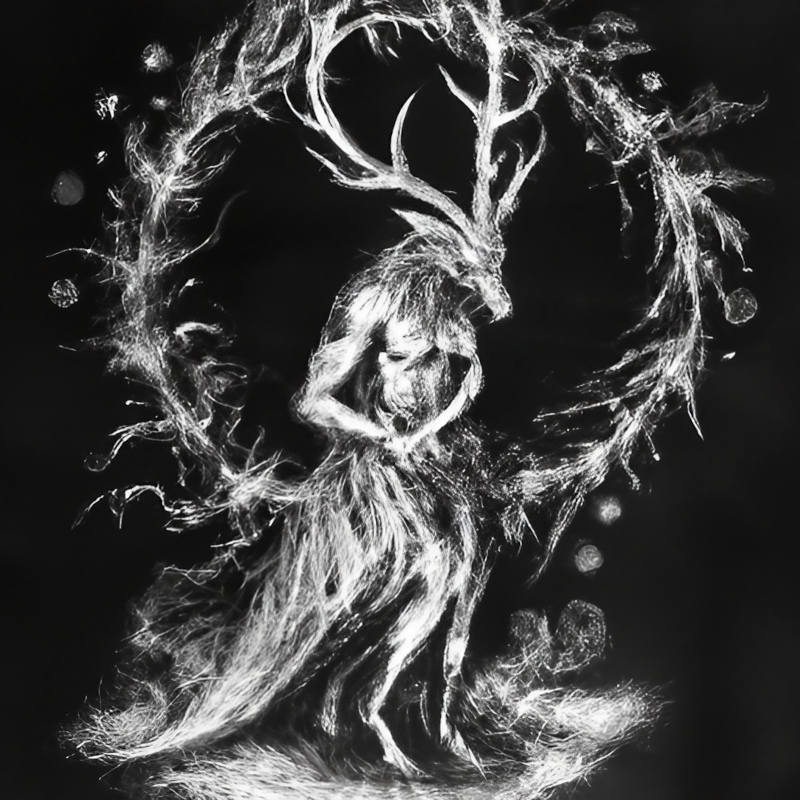
\includegraphics[scale=.5]{remembrance/SprigganBottom}
\end{center}

\begin{multicols*}{2}
